% Options for packages loaded elsewhere
\PassOptionsToPackage{unicode}{hyperref}
\PassOptionsToPackage{hyphens}{url}
%
\documentclass[
]{article}
\usepackage{amsmath,amssymb}
\usepackage{iftex}
\ifPDFTeX
  \usepackage[T1]{fontenc}
  \usepackage[utf8]{inputenc}
  \usepackage{textcomp} % provide euro and other symbols
\else % if luatex or xetex
  \usepackage{unicode-math} % this also loads fontspec
  \defaultfontfeatures{Scale=MatchLowercase}
  \defaultfontfeatures[\rmfamily]{Ligatures=TeX,Scale=1}
\fi
\usepackage{lmodern}
\ifPDFTeX\else
  % xetex/luatex font selection
\fi
% Use upquote if available, for straight quotes in verbatim environments
\IfFileExists{upquote.sty}{\usepackage{upquote}}{}
\IfFileExists{microtype.sty}{% use microtype if available
  \usepackage[]{microtype}
  \UseMicrotypeSet[protrusion]{basicmath} % disable protrusion for tt fonts
}{}
\makeatletter
\@ifundefined{KOMAClassName}{% if non-KOMA class
  \IfFileExists{parskip.sty}{%
    \usepackage{parskip}
  }{% else
    \setlength{\parindent}{0pt}
    \setlength{\parskip}{6pt plus 2pt minus 1pt}}
}{% if KOMA class
  \KOMAoptions{parskip=half}}
\makeatother
\usepackage{xcolor}
\usepackage[margin=1in]{geometry}
\usepackage{color}
\usepackage{fancyvrb}
\newcommand{\VerbBar}{|}
\newcommand{\VERB}{\Verb[commandchars=\\\{\}]}
\DefineVerbatimEnvironment{Highlighting}{Verbatim}{commandchars=\\\{\}}
% Add ',fontsize=\small' for more characters per line
\usepackage{framed}
\definecolor{shadecolor}{RGB}{248,248,248}
\newenvironment{Shaded}{\begin{snugshade}}{\end{snugshade}}
\newcommand{\AlertTok}[1]{\textcolor[rgb]{0.94,0.16,0.16}{#1}}
\newcommand{\AnnotationTok}[1]{\textcolor[rgb]{0.56,0.35,0.01}{\textbf{\textit{#1}}}}
\newcommand{\AttributeTok}[1]{\textcolor[rgb]{0.13,0.29,0.53}{#1}}
\newcommand{\BaseNTok}[1]{\textcolor[rgb]{0.00,0.00,0.81}{#1}}
\newcommand{\BuiltInTok}[1]{#1}
\newcommand{\CharTok}[1]{\textcolor[rgb]{0.31,0.60,0.02}{#1}}
\newcommand{\CommentTok}[1]{\textcolor[rgb]{0.56,0.35,0.01}{\textit{#1}}}
\newcommand{\CommentVarTok}[1]{\textcolor[rgb]{0.56,0.35,0.01}{\textbf{\textit{#1}}}}
\newcommand{\ConstantTok}[1]{\textcolor[rgb]{0.56,0.35,0.01}{#1}}
\newcommand{\ControlFlowTok}[1]{\textcolor[rgb]{0.13,0.29,0.53}{\textbf{#1}}}
\newcommand{\DataTypeTok}[1]{\textcolor[rgb]{0.13,0.29,0.53}{#1}}
\newcommand{\DecValTok}[1]{\textcolor[rgb]{0.00,0.00,0.81}{#1}}
\newcommand{\DocumentationTok}[1]{\textcolor[rgb]{0.56,0.35,0.01}{\textbf{\textit{#1}}}}
\newcommand{\ErrorTok}[1]{\textcolor[rgb]{0.64,0.00,0.00}{\textbf{#1}}}
\newcommand{\ExtensionTok}[1]{#1}
\newcommand{\FloatTok}[1]{\textcolor[rgb]{0.00,0.00,0.81}{#1}}
\newcommand{\FunctionTok}[1]{\textcolor[rgb]{0.13,0.29,0.53}{\textbf{#1}}}
\newcommand{\ImportTok}[1]{#1}
\newcommand{\InformationTok}[1]{\textcolor[rgb]{0.56,0.35,0.01}{\textbf{\textit{#1}}}}
\newcommand{\KeywordTok}[1]{\textcolor[rgb]{0.13,0.29,0.53}{\textbf{#1}}}
\newcommand{\NormalTok}[1]{#1}
\newcommand{\OperatorTok}[1]{\textcolor[rgb]{0.81,0.36,0.00}{\textbf{#1}}}
\newcommand{\OtherTok}[1]{\textcolor[rgb]{0.56,0.35,0.01}{#1}}
\newcommand{\PreprocessorTok}[1]{\textcolor[rgb]{0.56,0.35,0.01}{\textit{#1}}}
\newcommand{\RegionMarkerTok}[1]{#1}
\newcommand{\SpecialCharTok}[1]{\textcolor[rgb]{0.81,0.36,0.00}{\textbf{#1}}}
\newcommand{\SpecialStringTok}[1]{\textcolor[rgb]{0.31,0.60,0.02}{#1}}
\newcommand{\StringTok}[1]{\textcolor[rgb]{0.31,0.60,0.02}{#1}}
\newcommand{\VariableTok}[1]{\textcolor[rgb]{0.00,0.00,0.00}{#1}}
\newcommand{\VerbatimStringTok}[1]{\textcolor[rgb]{0.31,0.60,0.02}{#1}}
\newcommand{\WarningTok}[1]{\textcolor[rgb]{0.56,0.35,0.01}{\textbf{\textit{#1}}}}
\usepackage{graphicx}
\makeatletter
\def\maxwidth{\ifdim\Gin@nat@width>\linewidth\linewidth\else\Gin@nat@width\fi}
\def\maxheight{\ifdim\Gin@nat@height>\textheight\textheight\else\Gin@nat@height\fi}
\makeatother
% Scale images if necessary, so that they will not overflow the page
% margins by default, and it is still possible to overwrite the defaults
% using explicit options in \includegraphics[width, height, ...]{}
\setkeys{Gin}{width=\maxwidth,height=\maxheight,keepaspectratio}
% Set default figure placement to htbp
\makeatletter
\def\fps@figure{htbp}
\makeatother
\setlength{\emergencystretch}{3em} % prevent overfull lines
\providecommand{\tightlist}{%
  \setlength{\itemsep}{0pt}\setlength{\parskip}{0pt}}
\setcounter{secnumdepth}{-\maxdimen} % remove section numbering
\ifLuaTeX
  \usepackage{selnolig}  % disable illegal ligatures
\fi
\usepackage{bookmark}
\IfFileExists{xurl.sty}{\usepackage{xurl}}{} % add URL line breaks if available
\urlstyle{same}
\hypersetup{
  pdftitle={31\_DataVisualization},
  pdfauthor={Melody Lu, Chiko Orji, Ananya Pandit},
  hidelinks,
  pdfcreator={LaTeX via pandoc}}

\title{31\_DataVisualization}
\author{Melody Lu, Chiko Orji, Ananya Pandit}
\date{2025-11-08}

\begin{document}
\maketitle

\begin{Shaded}
\begin{Highlighting}[]
\FunctionTok{file.info}\NormalTok{(}\StringTok{"01vis\_q2"}\NormalTok{)}
\end{Highlighting}
\end{Shaded}

\begin{verbatim}
##           size isdir mode               mtime               ctime
## 01vis_q2 67792 FALSE  644 2025-12-05 23:46:40 2025-12-05 23:46:40
##                        atime uid gid     uname grname
## 01vis_q2 2025-12-05 23:51:12 501  20 chikoorji  staff
\end{verbatim}

\begin{Shaded}
\begin{Highlighting}[]
\FunctionTok{source}\NormalTok{(}\StringTok{"01\_datacleaning.R"}\NormalTok{)}
\end{Highlighting}
\end{Shaded}

\begin{verbatim}
## -- Attaching core tidyverse packages ------------------------ tidyverse 2.0.0 --
## v dplyr     1.1.4     v readr     2.1.5
## v forcats   1.0.1     v stringr   1.5.1
## v ggplot2   3.5.2     v tibble    3.2.1
## v lubridate 1.9.4     v tidyr     1.3.1
## v purrr     1.1.0     
## -- Conflicts ------------------------------------------ tidyverse_conflicts() --
## x dplyr::filter() masks stats::filter()
## x dplyr::lag()    masks stats::lag()
## i Use the conflicted package (<http://conflicted.r-lib.org/>) to force all conflicts to become errors
## 
## Attaching package: 'janitor'
## 
## 
## The following objects are masked from 'package:stats':
## 
##     chisq.test, fisher.test
## 
## 
## Rows: 144 Columns: 22
## -- Column specification --------------------------------------------------------
## Delimiter: ","
## chr  (1): chamber
## dbl (21): congress, year, party.mean.diff.d1, prop.moderate.d1, prop.moderat...
## 
## i Use `spec()` to retrieve the full column specification for this data.
## i Specify the column types or set `show_col_types = FALSE` to quiet this message.
## Rows: 774 Columns: 25
## -- Column specification --------------------------------------------------------
## Delimiter: ","
## chr (24): Candidate, State, District, Office Type, Race Type, Race Primary E...
## dbl  (1): Primary %
## 
## i Use `spec()` to retrieve the full column specification for this data.
## i Specify the column types or set `show_col_types = FALSE` to quiet this message.
\end{verbatim}

\begin{verbatim}
## Warning: One or more parsing issues, call `problems()` on your data frame for details,
## e.g.:
##   dat <- vroom(...)
##   problems(dat)
\end{verbatim}

\begin{verbatim}
## Rows: 1599 Columns: 27
## -- Column specification --------------------------------------------------------
## Delimiter: ","
## chr (26): Candidate, Gender, Race 1, Race 2, Incumbent, Incumbent Challenger...
## lgl  (1): Race 3
## 
## i Use `spec()` to retrieve the full column specification for this data.
## i Specify the column types or set `show_col_types = FALSE` to quiet this message.
## Rows: 811 Columns: 32
## -- Column specification --------------------------------------------------------
## Delimiter: ","
## chr (30): Candidate, State, District, Office Type, Race Type, Race Primary E...
## dbl  (2): Partisan Lean, Primary %
## 
## i Use `spec()` to retrieve the full column specification for this data.
## i Specify the column types or set `show_col_types = FALSE` to quiet this message.
## Rows: 1077 Columns: 26
## -- Column specification --------------------------------------------------------
## Delimiter: ","
## chr (26): Candidate, Gender, Race 1, Race 2, Race 3, Incumbent, Incumbent Ch...
## 
## i Use `spec()` to retrieve the full column specification for this data.
## i Specify the column types or set `show_col_types = FALSE` to quiet this message.
\end{verbatim}

TITLE: How Demographics and Party Dynamics Shape Primaries

\section{ABSTRACT:}\label{abstract}

This project explores how party dynamics and candidate demographics
relate to primary election success in the United States. Using statewide
Democratic and Republican primary candidate data from the 2022 election
cycle, we examine the relationships between gender, race, party, and
office type in shaping who wins and who loses. Our visualizations show
that gender on its own is not a strong or consistent predictor of
success, but once the data is separated by party and office type, clear
differences begin to emerge.

Women tend to perform better than men in Democratic primaries, while men
continue to dominate Republican primaries, especially in more
competitive Senate contests. Race also interacts with these patterns,
and some gender--race combinations experience stronger or weaker
outcomes depending on the political environment. Our logistic regression
results confirm that primary vote percentage is the single strongest
factor in determining who wins a primary, but even after controlling for
vote share, party and race still show meaningful associations with
outcomes.

A secondary question on ideology changes will be further explored to
understand how differences in ideological positioning relate to these
structural patterns. We also look at ideology to see whether being more
moderate or more extreme affects a candidate's chances of winning. Early
patterns show that ideology might matter differently for different
groups. For example, some gender--race combinations seem to do better
when they are closer to the party's mainstream, while others face more
challenges when they take more ideological positions.

\section{INTRO:}\label{intro}

The purpose of this study is to understand how gender, race, and
ideological placement relate to political success in U.S. primary
elections and to see how these patterns differ between Democrats and
Republicans. Primary elections play a major role in determining who
appears on the general election ballot, so studying who wins primaries
can tell us a lot about representation, competitiveness, and the types
of candidates each party tends to reward.

The first research question we explore asks how gender correlates with
primary win rates and whether this relationship is different across
parties or office types such as Governor and Senate. Past research
suggests that gender and race can influence electoral outcomes, but
these effects often depend heavily on the political context, making it
important to examine Democrats and Republicans separately. The second
research question, which will be addressed later, will focus on ideology
by looking at how ideological differences between parties relate to
broader dynamics in primary competitiveness. Throughout the report, we
use a mix of visualizations and logistic regression models to identify
where demographic traits matter most and where larger structural
patterns shape election outcomes.

The second research question we explore looks at ideology and how the
ideological positions of the two major parties have changed over time.
To examine this, we use two visualizations: one that shows how much the
ideological distributions of Democrats and Republicans overlap from year
to year, and another that tracks the growing ideological distance
between the parties. These graphs help us see whether increasing
polarization shapes primary competitiveness and whether candidates are
rewarded for aligning more closely with their party's ideological center
or its extremes.

\section{DATA:}\label{data}

The dataset consists of all Democratic and Republican statewide primary
candidates from the 2022 election cycle. Each row represents a candidate
and includes information about the candidate's gender, race, party
affiliation, office sought (Senate or Governor), primary vote
percentage, and primary outcome. The dataset also includes ideological
scores that will be used later in the second part of the project. The
2022 cycle offers a large and balanced sample across both parties,
making it a strong foundation for exploring demographic differences in
performance and success.

For the second dataset, which tracks ideological polarization in
Congress over time, we used the provided file containing yearly ideology
scores for Democratic and Republican legislators. This dataset includes
measures such as party means, ideological spread, and distance between
the parties in each year.

\section{DATA CLEANING:}\label{data-cleaning}

To prepare the dataset for analysis, we followed a strong cleaning
process. Missing or inconsistent demographic information was removed to
ensure fair comparisons. Gender labels were standardized into
``Female,'' ``Male,'' and ``Nonbinary,'' and primary election outcomes
were standardized into a binary format showing if the candidate won (1)
or lost (0). Because this project focuses specifically on the two major
political parties, we filtered out minor-party candidates. Primary vote
percentages, which appear in different formats in the raw data, were
converted into numeric values so they could be used directly in the
regression model. We also created grouped data structures that combine
race, gender, party, and office type, which allowed us to build heatmaps
and intersectional analyses later in the report. These steps ensured
that the dataset was clean, consistent, and ready for both visual and
statistical modeling.

For the second dataset, we cleaned the data by selecting the variables
needed for our two visualizations---overlap between the parties and
ideological distance over time standardizing column names, and removing
years with incomplete information. We also converted party labels and
ideology values into a consistent numeric format so the trends could be
plotted clearly. This cleaned dataset allowed us to create the two
graphs used in the ideology section and to compare long-term ideological
change to the patterns we observed in the primary candidate data.

VISUALIZATION 1: Win Rate by Gender and Party

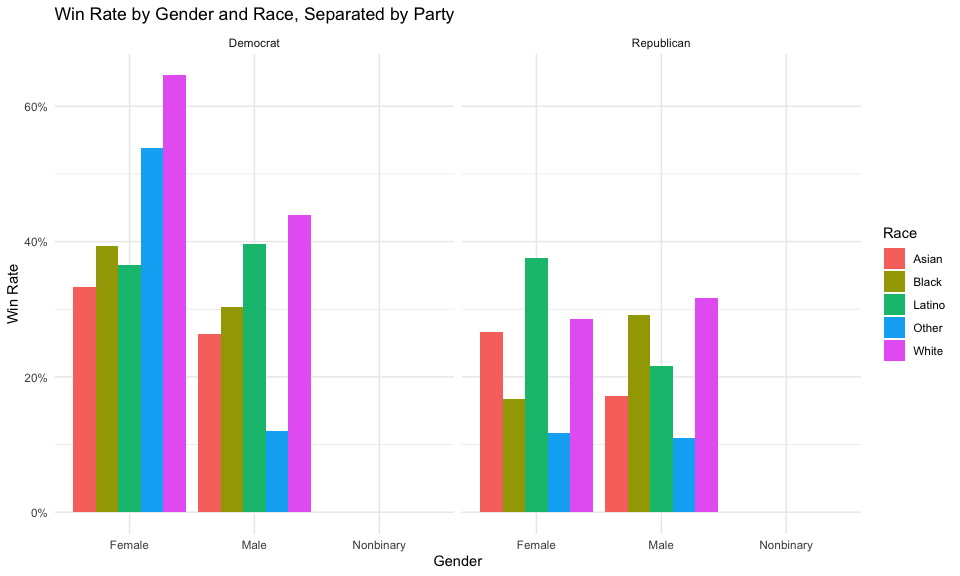
\includegraphics[width=0.7\linewidth]{winrate_gender_rate_party}

When we look at win rates by gender across the entire dataset, the
differences aren't large. However, once we split the results by
political party, the patterns become much clearer.

In Democratic primaries, women tend to win at higher rates than men.
This could reflect a combination of factors, such as Democratic voters
being more willing to support women, a lot more greater institutional
encouragement inside the Democratic Party for women to run, or women
being more selective and entering races where they know they have
stronger chances of success.

In Republican primaries, the trend is the opposite. Men win far more
often than women, which may potentially reflect deeper structural
differences within the party, such as fewer women being recruited, fewer
women receiving financial support, or ideological currents within
Republican politics that may make it more difficult for women to gain
traction in primaries. The giant contrast between the two parties shows
that gender effects are not uniform. Instead, gender interacts heavily
with party culture, different recruitment pipelines, the competitiveness
of candidate pools, and the types of candidates each party tends to
reward.

Visualization 2: Distribution of Primary Vote Percentage by Gender

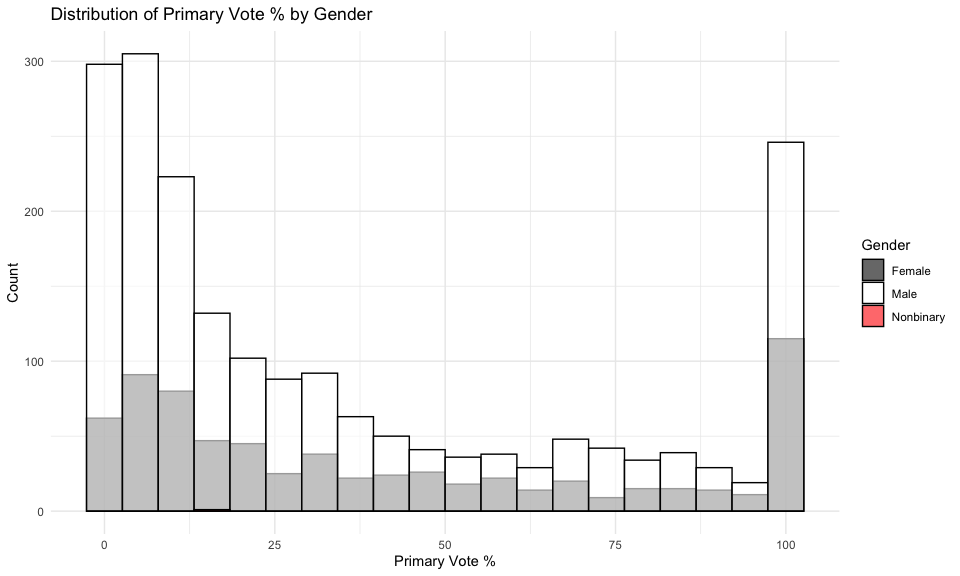
\includegraphics[width=0.7\linewidth]{distribution_primaryvote_gender}

Looking at how primary vote percentages are distributed across genders
helps us understand not just who wins but how candidates perform
overall. The histogram shows that female candidates tend to cluster more
in the mid-to-high range of vote percentages, meaning that even when
women don't win, they tend to remain competitive throughout the race.

Male candidates show a much wider spread, including both extremely
strong performances and a larger number of poor-performing campaigns.
This suggests that men enter a larger variety of races, some of which
may be unwinnable, whereas women may be more strategic or may face more
structural filtering before entering a race.

Nonbinary candidates appear too infrequently for meaningful comparison,
but their limited presence reflects broader patterns in statewide
politics. While the differences in distribution are not extreme, they do
suggest that women tend to run more consistently strong campaigns
overall, while men run in a wider variety of campaign contexts with more
variability in performance.

Visualization 3: Primary Win Rate by Race X Gender X Party

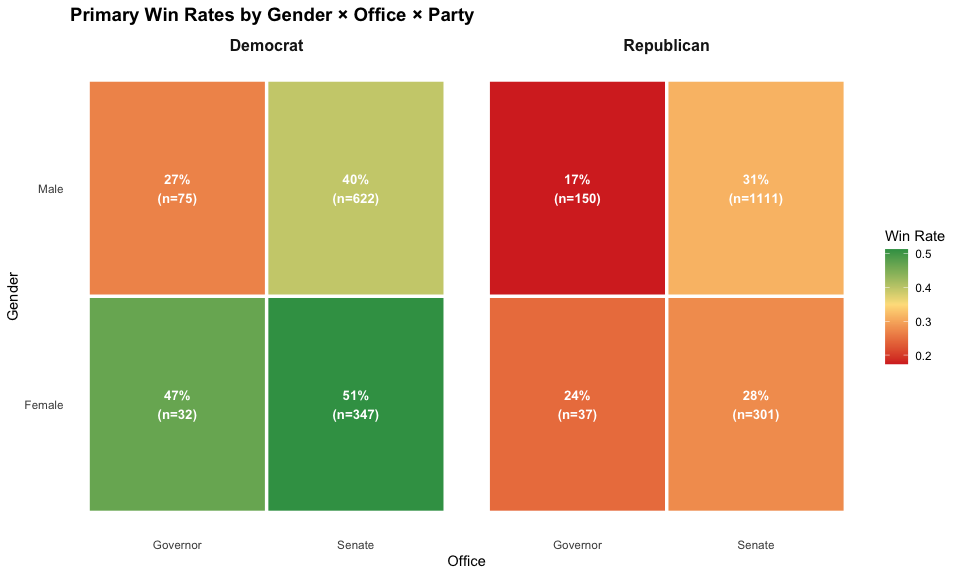
\includegraphics[width=0.7\linewidth]{pwr_gender_race_party}

Race adds another important layer to understanding primary outcomes.

When we examine win rates across racial groups alone, we see that White
and Black candidates tend to have higher success rates, Asian candidates
fall in the middle, and Latino or ``Other'' candidates have somewhat
lower success rates.

However, these overall averages don't tell the full story because the
role of race becomes clearer when we combine it with gender.

In intersectional visualizations, White women tend to perform especially
well in Democratic primaries, and Black women also show relatively
strong success rates, though with smaller sample sizes. Latino men, on
the other hand, show lower win rates across both parties. These patterns
become even more pronounced when we separate results by party. In
Democratic primaries, racial gaps are smaller, and women of different
racial backgrounds win at relatively similar rates.

In Republican primaries, the gaps widen significantly, with White men
dominating success rates and most other racial and gender groups
experiencing lower outcomes. These findings reflect broader political
dynamics in the United States, where the Democratic Party tends to field
a more diverse set of candidates and has voters more willing to support
racial and gender diversity, while the Republican Party tends to favor
candidates who align more closely with its historically White, male base
of primary voters.

Visualization 4: Win Rates by Office Type: Senate vs Governor

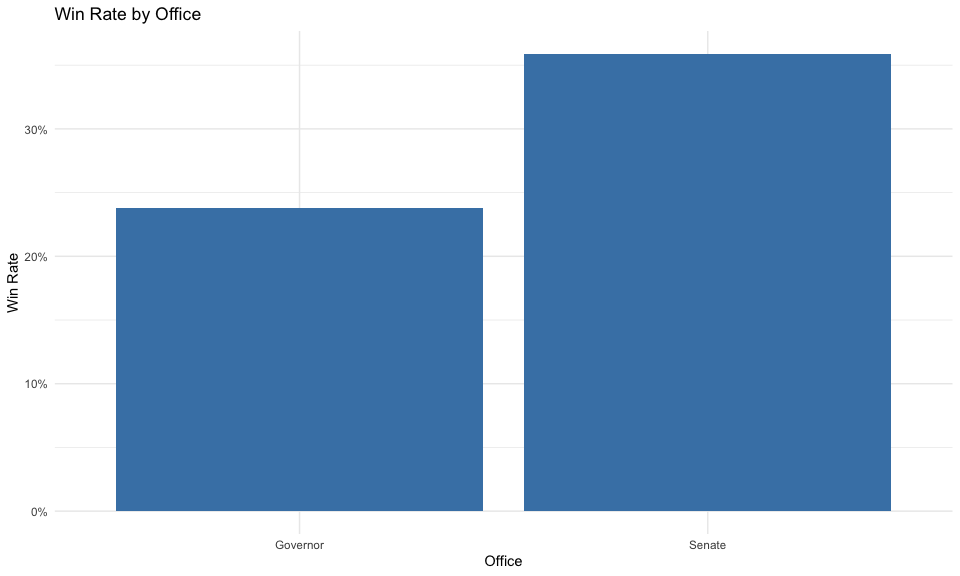
\includegraphics[width=0.7\linewidth]{winrate_office}

Office type also plays a major role in shaping primary outcomes. Senate
races tend to be more competitive because they attract larger pools of
candidates, have much higher stakes, and typically involve fewer seats.
As a result, the overall win rates in Senate races are lower, simply
because candidates face more competition.

Governor races, on the other hand, often have clearer frontrunners,
fewer challengers, and more defined party support structures, which
leads to higher average win rates. Because women and men do not enter
each office type at the same rate, these structural differences can
contribute to gender gaps.

If women are more likely to run for Senate seats, where success rates
are naturally lower, their overall win rates may appear worse even if
they perform just as competitively within their own office category.
Understanding office type is important because it highlights how
structural competitiveness and not just demographic traits shapes
electoral outcomes.

Visualization 5: Heatmap: Gender × Office × Party

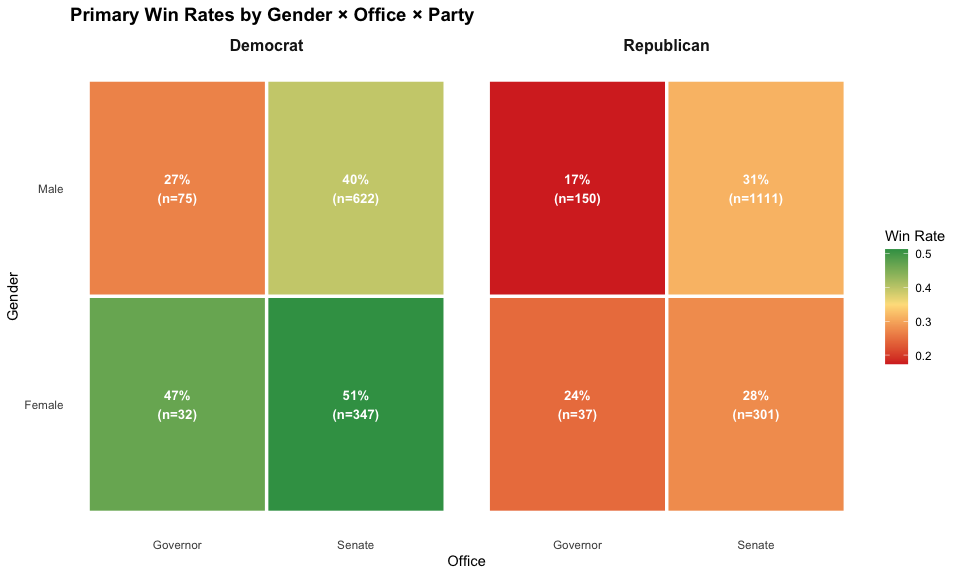
\includegraphics[width=0.7\linewidth]{pwr_gender_race_party}

The heatmap brings together gender, office type, and party into a single
visualization, and it is one of the most interesting figures in the
analysis.

In Democratic primaries, women show consistently strong success rates
across both Governor and Senate races. Men also perform well, but women
often hold a slight advantage, suggesting that Democratic voters and
institutions may be more favorable environments for female candidates.

In Republican primaries, this pattern flips. Women consistently show
lower success rates across both offices, but especially in Senate
contests, where the gender gap widens substantially. Men continue to
dominate across most Republican categories. What makes the heatmap so
strong is that it shows how gender differences are not simply ``men do
better'' or ``women do better.'' Instead, the relationship depends on
the interaction of three major structural factors: the political
environment of the party, the level of competitiveness of the office,
and the gender composition of the candidate pool. These combinations
help explain the earlier results and clarify why gender alone is not a
consistent predictor of success.

Visualization: Logistic Regression: Main Predictors of Winning

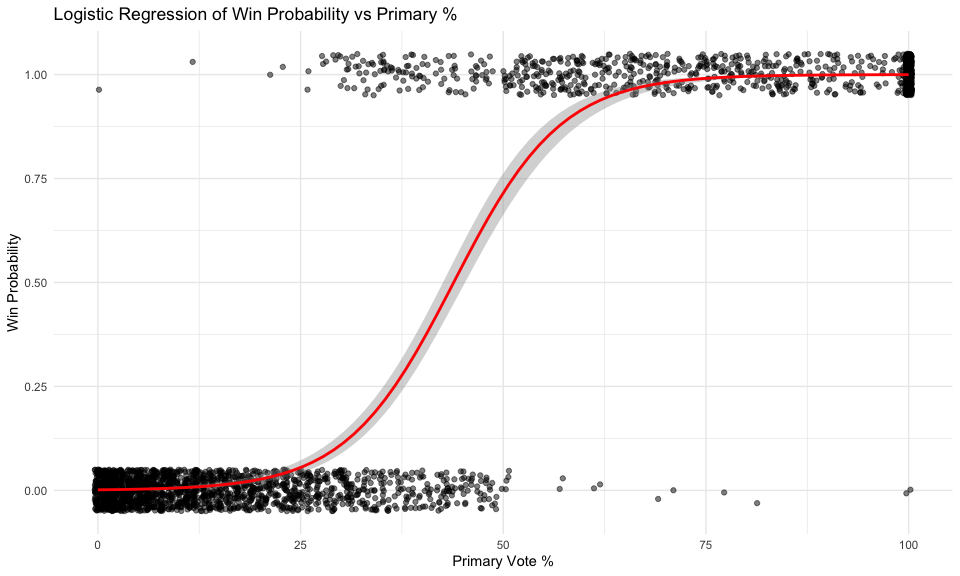
\includegraphics[width=0.7\linewidth]{logistic_regression_win}
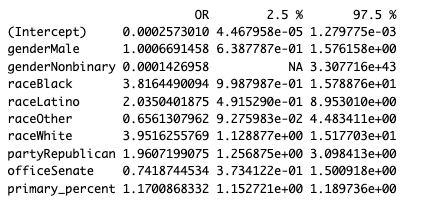
\includegraphics[width=0.7\linewidth]{logistic_reg}

The logistic regression model tests whether gender still matters after
controlling for other important predictors such as party, race, office
type, and primary vote percentage. The results show that primary vote
percentage is by far the strongest predictor of winning, which makes
more logical sense because candidates who receive more votes are
overwhelmingly the ones who win. In fact, each additional percentage
point of vote share significantly increases a candidate's odds of
victory. The party also remains important, with Republican candidates
showing higher odds of winning, more likely because Republican primaries
in this dataset tend to have fewer candidates per race. After
controlling for vote share and party, gender itself is not statistically
significant, meaning that gender does not independently determine the
likelihood of winning.

Race shows some associations with win probability, but the estimates
come with uncertainty due to sample size differences. Office type
continues to matter as well, with Senate candidates having slightly
lower odds relative to Governor candidates, echoing the earlier
observation that Senate races are more competitive.

The regression results confirm that the raw gender gaps seen in the
visualizations arise mostly from contextual differences such as party
environments, competitiveness, and candidate pool composition rather
than gender acting as a direct causal factor.

VISUALIZATION: IDEOLOGICAL OVERLAP IN CONGRESS

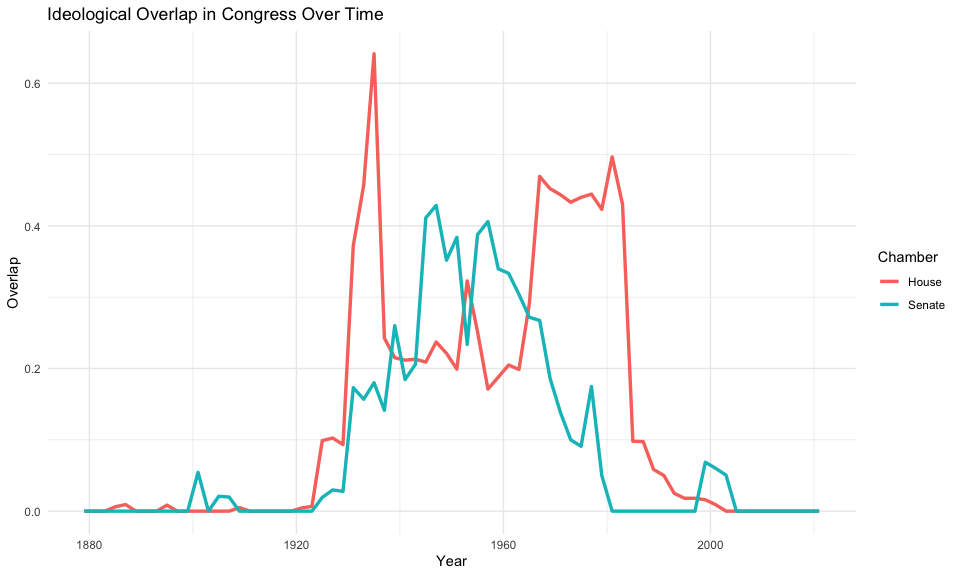
\includegraphics[width=0.7\linewidth]{01vis_q2}

The first plot shows how far apart Democrats and Republicans are
ideologically in the House and Senate from the late 1800s to today.
Higher values mean the parties are more polarized --- their average
ideological positions are farther apart. The patterns show that
polarization dropped sharply around the mid-20th century, reaching its
lowest point between the 1940s and 1950s, when the parties were the most
ideologically similar. After roughly 1970, the distance between the
parties begins rising steadily in both chambers, with the modern era
showing the highest levels of polarization on record. The House
consistently polarizes earlier and more sharply than the Senate.
Overall, this visualization makes it clear that Congress has become
dramatically more polarized over time, especially since the 1980s.

VISUALIZATION:

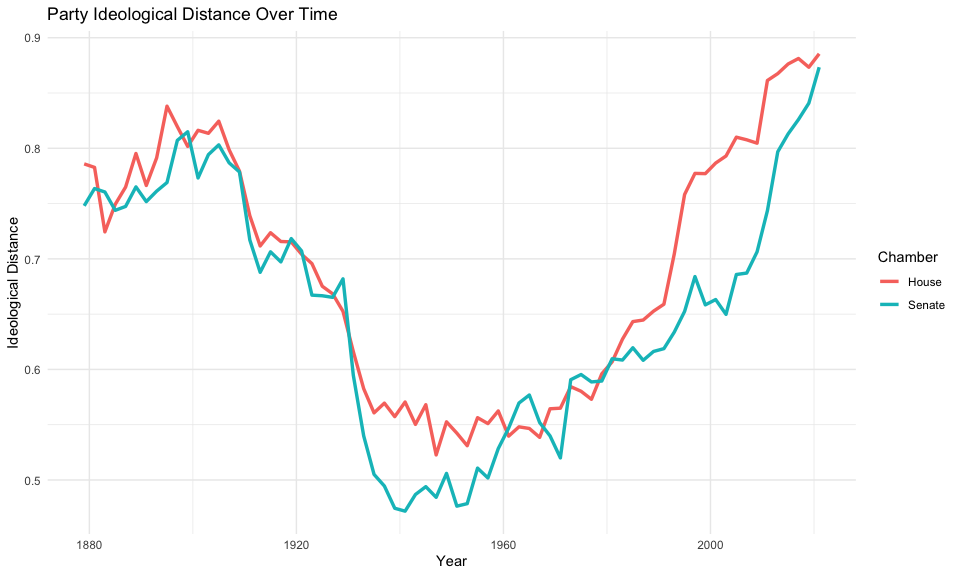
\includegraphics[width=0.7\linewidth]{02_visq2}

The second plot flips the perspective by showing overlap---the amount of
shared ideological space between Democrats and Republicans. Higher
values mean the parties have members who vote similarly; lower values
mean there is almost no ideological mixing. Early in U.S. history,
overlap was relatively high, especially in moments where conservative
Democrats and liberal Republicans existed. Overlap peaked around the
1920s--1940s, but then fell sharply beginning in the 1970s. Today,
overlap is essentially zero, meaning the parties no longer share any
meaningful ideological common ground. The House loses its overlap
slightly faster than the Senate, but both chambers ultimately converge
to the same place: near-total separation. This visualization reinforces
the story from the first plot --- modern Congress is defined by extreme
partisan separation, with almost no ideological crossover remaining.

\section{Conclusion:}\label{conclusion}

Overall, this project shows that gender does correlate with primary
election success, but the relationship isn't straightforward. Instead,
the effect of gender depends heavily on the political and structural
environment surrounding each candidate. Women tend to perform better in
Democratic primaries, while men perform better in Republican primaries,
particularly in competitive Senate races. These differences reveal how
party culture, recruitment patterns, and voter preferences shape who
succeeds. Office type also matters, with Senate races showing lower
success rates because they attract more crowded and competitive fields.

Race introduces additional layers, as certain gender--race combinations
show stronger or weaker outcomes depending on party context. Our
logistic regression confirms that vote share is the dominant predictor
of winning, and once we account for vote share and party, gender itself
no longer predicts outcomes by itself.

This means that most gender differences come from structural factors:
who runs, which offices they run for, and the dynamics of each party,
rather than gender acting as a direct barrier or advantage. These
findings highlight the importance of studying election outcomes in
context rather than in isolation.

The ideology results support this argument by showing how the broader
political environment has changed over time. The ideological distance
between Democrats and Republicans has grown dramatically since the
1970s, while ideological overlap has nearly disappeared. This long-term
polarization helps explain why party differences in primary outcomes are
so strong today: candidates operate in a system where the parties are
farther apart than ever, leaving little shared ideological space. As
polarization increases, party context becomes even more influential in
shaping which types of candidates succeed.

Group Contributions: Chiko - Data Cleaning, Visualizations for Question
1/2, Coding Ananya - Report, Coding Melody - Coding, Visualizations for
Question 2

\end{document}
